\documentclass{article}
\usepackage[left=2cm,right=2cm,
    top=2cm,bottom=2cm,bindingoffset=0cm]{geometry}
\usepackage[T2A]{fontenc}
\usepackage[utf8]{inputenc}
\usepackage[english,russian]{babel}
\usepackage{indentfirst}
\usepackage[final]{graphicx}
\usepackage{algorithm}
\usepackage{algorithmic}
\usepackage{multirow}
\usepackage{longtable}
\usepackage{tabulary}
\usepackage{placeins}
\usepackage{needspace}
\usepackage{color}

\usepackage{listings}

\lstset{
	language = Haskell,
  frame=none,
  xleftmargin=2pt,
  stepnumber=1,
  numbers=left,
  numbersep=5pt,
  numberstyle=\ttfamily\tiny\color[gray]{0.3},
  belowcaptionskip=\bigskipamount,
  captionpos=b,
  escapeinside={*'}{'*},
  tabsize=2,
  emphstyle={\bf},
  commentstyle=\it,
  stringstyle=\mdseries\rmfamily,
  showspaces=false,
  keywordstyle=\bfseries\rmfamily,
  columns=flexible,
  basicstyle=\small\sffamily,
  showstringspaces=false,
  morecomment=[l]\%,
}

\usepackage{wrapfig}
\graphicspath{{Images/}}
\DeclareGraphicsExtensions{.pdf,.png,.jpg,.svg}

\renewcommand{\labelenumi}{\arabic{enumi}.}
\renewcommand{\labelenumii}{\asbuk{enumii})}

\lstset{language=C++,
                basicstyle=\ttfamily,
                keywordstyle=\color{blue}\ttfamily,
                stringstyle=\color{red}\ttfamily,
                commentstyle=\color{green}\ttfamily,
                morecomment=[l][\color{magenta}]{\#}
}


%Images
\usepackage{graphicx}
\DeclareGraphicsExtensions{.pdf,.png,.jpg}
\usepackage{wrapfig}
\renewcommand{\thefigure}{\thesection.\arabic{figure}}
\renewcommand{\thetable}{\thesection.\arabic{figure}}

\author{Пахтусов Н. Г., ПРО-306}
\makeatletter

%Roman num
\newcommand*{\rom}[1]{\expandafter\@slowromancap\romannumeral #1@}

\begin{document}

\begin{center}
\thispagestyle{empty} 

Федеральное государственное бюджетное образовательное учереждение высшего \\
профессионального образования\\
<<Уфимский государственный авиационный технический университет>>
\vspace*{\fill}
\begingroup
\centering

Пояснительная записка к курсовой работе\\
по дисциплине <<Методы вычислений>>\\
<<Поиск корней функции одного аргумента>>

\endgroup
\vspace*{\fill}

\end{center}

\begin{flushright}

Выполнил:\\
\@author \\
Проверила:\\
Гадилова Ф. Г.

\end{flushright}

\begin{center}
$\bullet$ Уфа, 2015
\end{center}

\clearpage

\tableofcontents

\clearpage

\section{Введение}

\section{Постановка задачи}

	Пусть задана функция f(x) действительной переменной. Требуется найти корни уравнения:\\
	
	\texttt{f(x)=0.} (1)
	
	

\section{Теория}

	Задача нахождения корней уравнения (1) обычно решается в 2 этапа. На первом этапе проводится отделение корней, т.е. выделение отрезков, содержащих только один корень. На втором этапе, используя начальное приближение, строится итерационный процесс, позволяющий уточнить значение отыскиваемого корня.

	Для того, чтобы найти корни функций одного аргумента, можно использовать множество методов.
	
		\subsection{Интерполяция для решения уравнений}
		
			Рассмотрим методы решения уравнения f(x) = 0 с помощью применения интерполяции. Выясним, есть ли преимущества при замене исходной функции на интерполяционную функцию, и какова точность нахождения корня при переходе к решению интерполяционного уравнения.
			
			\subsubsection{Постановка задачи}
			
				Пусть на отрезке \texttt{[a,b]} задана функция \texttt{f(x)}, и необходимо решить уравнение \texttt{f(x) = 0} на этом отрезке. Известно много различных способов нахождения корней уравнения, но мы поступим следующим образом: будем приближать исходную функцию \texttt{f(x)} другой функцией \texttt{(x)} и искать корни именно интерполированной (в англоязычной аббревиатуре -- \textbf{Interpolation}) функции \texttt{g(x)}.
				
				Рассмотрим следующие методы интерполяции:
				
				\begin{itemize}
					\item Интерполяция каноническим полиномом
					\item Интерполяция полиномами Лагранжа
					\item Интерполяция степенными рядами
					\item Интерполяция кубическими сплайнами
					\item Тригонометрическая интерполяция
				\end{itemize}
				
			\subsubsection{Сравнение методов}
			
				\begin{wrapfigure}[18]{h}{0.4\linewidth} 
					\center{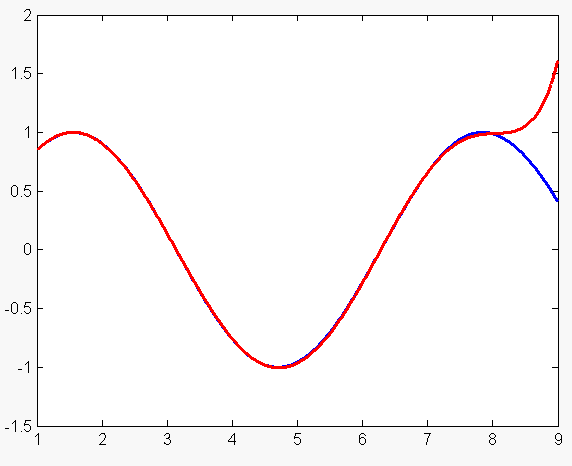
\includegraphics[width=\linewidth]{interpol1}}
					\caption{График синуса и интерполирующей функции}
					\label{fig:dix1}
				\end{wrapfigure}
			
				Сравним методы интерполяции функций и выясним, какой из них лучше использовать для нахождения корней уравнения \texttt{f(x) = 0} в конкретном случае. В конечном итоге предстоит определить, насколько точно корни уравнения \texttt{g(x) = 0} приближают корни уравнения \texttt{f(x) = 0}.\\
				
				\textbf{Интерполяция каноническим полиномом.}
				
				Рассмотрим в качестве функции \texttt{f(x) = sin(x)} на \texttt{[1, 8]}, а в качестве интерполируемой функции \texttt{g(x)} -- полином, имеющий вид: 
				
			\begin{center}	\texttt{$g(x) = P_n(x) = c_0 + c_1x + c_2x^2 + ... + c_nx^n$}
	\end{center}
	
				\begin{wrapfigure}[20]{h}{0.5\linewidth} 
					\center{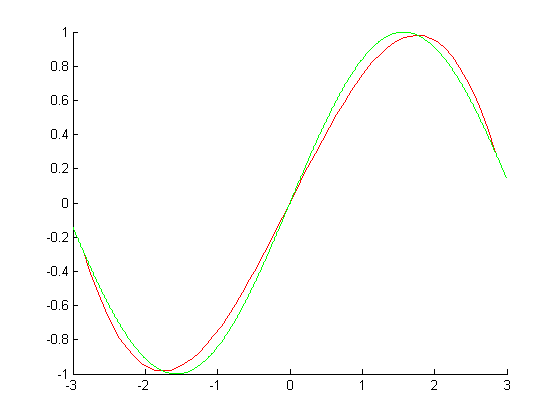
\includegraphics[width=\linewidth]	{interpol2}}
					\caption{График синуса и интерполирующей функции}
					\label{fig:dix2}
				\end{wrapfigure}
				
				В качестве узлов интерполяции выберем точки на отрезке \texttt{[1,8]} по алгоритму Чебышева. При выборе 8 узлов получается наименьшая ошибка интерполяции (она равна 0.0124).


								
				График синуса (показан синим цветом) и интерполирующей функции (показан красным цветом) в этом случае выглядит так (Рис. \ref{fig:dix1}).
		
				
				Корни полинома \texttt{g(x) = 0} будем искать, например, методом Гаусса. Ошибка при нахождении поиске складывается из ошибки интерполяции и ошибки решения уравнения.
				
				Погрешность интерполяции: \begin{center}$|R_n(x)| = \frac{M_{n+1}}{n + 1}\omega_n(x)$
				\end{center}
				Сложность метода Гаусса: $O(2\frac{n}{3})$.
				
				\textbf{Интерполяция полиномами Лагранжа.}
				
				Рассмотрим в качестве \texttt{f(x)} ту же функцию \texttt{sin(x)}, но на этот раз на отрезке \texttt{[-3,3]}, а в качестве интерполирующей функции \texttt{g(x)} рассмотрим полином: 
				
				\begin{center}\texttt{$P_n(x) = \sum\limits_{i=1}^ny_iQ_{n,i}(x)$}, где $Q_{n,i} = \prod\limits_{j = 0, j \neq i}^n \frac{x - x_j}{x_i - x_j}$.\end{center}
				
				В качестве узлов интерполяции снова по алгоритму Чебышева выберем точки на отрезке \texttt{[-3, 3]}.
				
				График синуса (показан красным цветом) и интерполирующей функции (показан зелёным цветом) в этом случае выглядит так (Рис. \ref{fig:dix2}).
				

				
				Уравнение Лагранжа \texttt{g(x) = 0} решается проще, чем \texttt{f(x) = 0}. При этом ошибка приближения: \texttt{0.0944}, погрешность интерполяции: \begin{center}$|R_n(x)| = \frac{f^{n+1}(\varepsilon)}{(n + 1)!}\omega_{n+1}(x)$.
				\end{center}
				Ошибка нахождения корней снова складывается из ошибки интерполяции и ошибки решения уравнения Лагранжа.
				
				\textbf{Интерполяция степенными рядами.}
				В качестве \texttt{f(x)} снова рассматриваем \texttt{sin(x)} на \texttt{[-1, 1]}, \texttt{g(x)} в данном случае имеет следующий вид: 
	\begin{center}			
				$g(x) = \sum\limits_{n=0}^{\infty}f^{(n)}(x_0)\frac{(x-x_0)^n}{n!}$\end{center}
				
				Графики показаны на Рис. \ref{fig:dix3}.
				
				Ошибка приближения в этом случае больше, поэтому данный метод интерполяции менее предпочтителен для поиска корней, погрешность интерполяции:\begin{center} $f(x) = f^{(n+1)}(\xi)\frac{(x-x_0)^{n+1}}{(n+1)!}$\\
				\end{center}
				\textbf{Интерполяция кубическими сплайнами.}
				
				\begin{wrapfigure}[13]{h}{0.5\linewidth} 
					\center{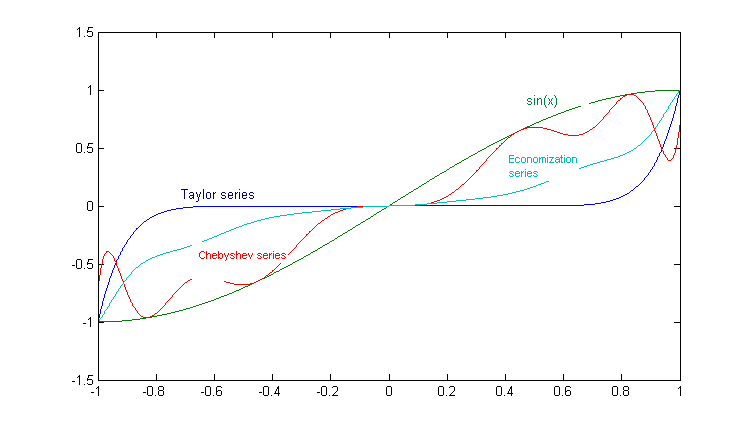
\includegraphics[width = \linewidth]	{interpol3}}
					\caption{График интерполяции степенными рядами}
					\label{fig:dix3}
				\end{wrapfigure}
				\texttt{f(x) = sin(x)} на \texttt{[-1, 1]}. \texttt{g(x)} -- сплайн-интерполяция синуса, функцию \texttt{f(x)} пытаемся представить в виде некоторых элементарных функций:
				
				\begin{center}$f(x)=\sum_{k=0}^N {c_k\Phi_k(x)},$\end{center} где $\{\Phi_k(x)\}$ -- фиксированный линейно независимые функции, $c_0, c_1, ... , c_n$ -- не определённые пока коэффициенты.
				
				
				
				При выборе шага \texttt{h = 0.25} интерполяция выглядит так (Рис. \ref{fig:dix4}).
				
				\begin{wrapfigure}[12]{H}{\linewidth}
					\center{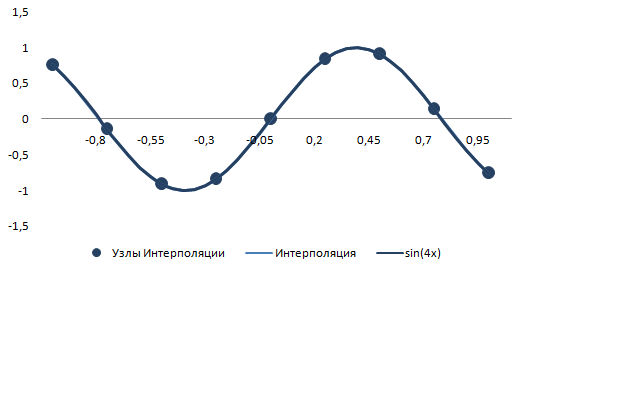
\includegraphics[width = \linewidth]{interpol4}}
					\label{fig:dix4}
				\end{wrapfigure}
				
				Ошибка интерполяции оценивается как \begin{center}$\parallel g-f\parallel \le \frac{5}{384}h^4\parallel \frac{d^4f}{df^4}\parallel$.\\\end{center}
				
				\textbf{Тригонометрическая интерполяция.}
				На этот раз разложим функцию f(x) (считаем её непрерывно-дифференцируемой) в ряд Фурье:
				
				\begin{center}$f(x)=\sum_{k=-\infty}^{\infty} \alpha_k exp^{2\pi i k x}$, где $\alpha_k=\int \limits_{0}^{1} f(x) exp {-2 \pi i k x} dx$.\end{center}
				
				Для её приближения будем использовать тригонометрический полином следующего вида: 
				
				$g(x) = F_n(x)=a_0 + a_1 \cos x + a_2 \cos 2x+\dots + a_n \cos nx + \\ \ + b_1 \sin x + b_2 \sin 2x+\dots + b_n \sin nx . $
				
				Тогда приближение функции f(x) функцией g(x) будет выглядеть примерно следующим образом (Рис. \ref{fig:dix5}):
				\begin{figure}[H]
					\center{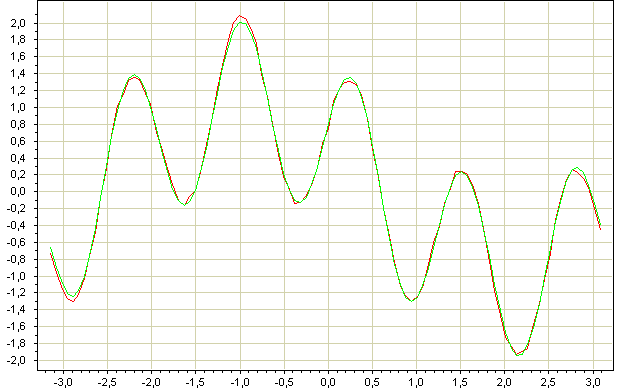
\includegraphics[width = \linewidth]	{interpol5}}
					\caption{График интерполяции степенными рядами}
					\label{fig:dix5}
				\end{figure}
				
				Поиск корней тригонометрической функции осуществляется итерационным методом. Анализ данного метода будет дан ниже.
				
			\subsubsection{Анализ методов}
			
				При решении уравнения f(x) = 0 вместо поиска корней исходной функции f(x) мы переходили к интерполирующей функции g(x) и искали её корни. Но какой же метод аппроксимации лучше для поиска корней?
Однозначного ответа на данный вопрос быть не может - это зависит от функции f(x). С одной стороны, надо использовать тот метод, который лучше приближает исходную функцию f(x). С другой стороны, мы должны достаточно точно отыскать корни g(x).

			Например, если сравнивать интерполяцию каноническим полиномом и полиномами Лагранжа, то лучше использовать второй метод, ибо он наиболее точно и с меньшими затратами приближает требуемую функцию, а сложность решения уравнения g(x) = 0 у них одинакова.

			А интерполяцию кубическими сплайнами рационально применять, если f(x) - периодическая или тригонометрическая функция. В случае приближения сплайнами, например, кусочно-линейной функции возникает следующий эффект (Рис. \ref{fig:dix6}):
			\begin{figure}{H}
					\center{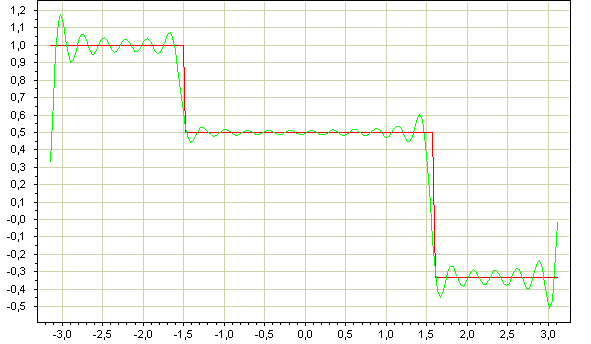
\includegraphics[width = \linewidth]	{interpol6}}
					\caption{График интерполяции степенными рядами}
					\label{fig:dix6}
			\end{figure}
			
			Понятно, что ни о какой точности решения уравнения g(x) = 0 говорить не приходится.
			
		\subsection{Методы дихотомии}
			
			\subsubsection{Введение}
			
				Существует довольно очевидная теорема: "Если непрерывная функция на концах некоторого интервала имеет значения разных знаков, то внутри этого интервала у нее есть корень (как минимум, один, но м.б. и несколько)". На базе этой теоремы построено численное нахождение приближенного значения корня функции. Обобщенно этот метод называется дихотомией, т.е. делением отрезка на две части. 
				
				Варианты метода дихотомии различаются выбором точки деления. Рассмотрим варианты дихотомии: \textbf{метод половинного деления} и \textbf{метод хорд}.\\
				
				\subsubsection{Метод половинного деления.}
				Метод половинного деления известен также как метод бисекции. В данном методе интервал делится ровно пополам.
				
				Такой подход обеспечивает гарантированную сходимость метода независимо от сложности функции - и это весьма важное свойство. Недостатком метода является то же самое - метод никогда не сойдется быстрее, т.е. сходимость метода всегда равна сходимости в наихудшем случае.\\
				
				\textbf{Изложение метода.}
				Перед применением метода для поиска корней функции необходимо отделить корни одним из известных способов, например, графическим методом. Отделение корней необходимо в случае, если неизвестно на каком отрезке нужно искать корень.

				Будем считать, что корень t функции f(x)=0 отделён на отрезке [a,b]. Задача заключается в том, чтобы найти и уточнить этот корень методом половинного деления. Другими словами, требуется найти приближённое значение корня с заданной точностью $\varepsilon$.
		
			Пусть функция f непрерывна на отрезке [a,b], $f(a)\cdot f(b)<0, \; \varepsilon=0,01$ и $t\in[a,b]$ -- единственный корень уравнения $f(x)=0, \; a\le t\le b$.
		
			(Мы не рассматриваем случай, когда корней на отрезке [a,b] несколько, то есть более одного. В качестве $\varepsilon$ можно взять и другое достаточно малое положительное число, например, 0,001.).
			Поделим отрезок [a,b] пополам. Получим точку $c= \frac {a+b}{2}, \; a<c<b$ и два отрезка $[a,c], \; [c,b]$.
			
			\begin{itemize}
				\item 
				Если $f(c)=0$ то корень  t найден (t = c). 
				\item 
				Если нет, то из двух полученных отрезков $[a,c]$ и $[c,b]$ надо выбрать один $[a_1;b_1]$ такой, что $f(a_1)\cdot f(b_1)<0$.
				
				Новый отрезок $[a_1;b_1]$ делим пополам. Получаем середину этого отрезка $c_1=\frac {a_1+b_1}{2}$ и так далее.
			
			\end{itemize}
			
			Для того, чтобы найти приближённое значение корня с точностью до $\varepsilon > 0$, необходимо остановить процесс половинного деления на таком шаге n>, на котором $|b_n-c_n|<\varepsilon$ и вычислить $x=\frac {a_n+b_n}{2}$. Тогда можно взять $t\approx x$.
			
			\subsubsection{Метод хорд}
			
				Недостаток деления отрезка строго пополам проистекает от того, что он использует лишь знак функции, игноририруя отклонение (абсолютную величину). Но очевидно, что чем меньше (по абсолютной величине) значение функции, тем ближе мы находимся к корню. Метод хорд предлагает делить отрезок в точке, отстоящей от краев отрезка пропорционально абсолютному значению функции на краях. (Название "метод хорд" происходит от того, что точка деления является пересечением отрезка $(X_{left},\; F(X_{left})), \; (X_{right},\; F(X_{right}))]$ -- хорды -- с осью абцисс.\\
			
				\textbf{Изложение метода.}
				Метод основан на замене функции f(x) на каждом шаге поиска хордой, пересечение которой с осью X дает приближение корня.
			
				При этом в процессе поиска семейство хорд может строиться:
				
				\begin{figure}{H}
					\center{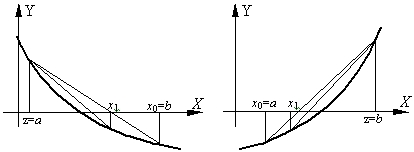
\includegraphics[width = \linewidth]	{interpol7}}
					\caption{График интерполяции степенными рядами}
					\label{fig:dix7}
				\end{figure}
				\begin{enumerate}
						\item 
						При фиксированном левом конце хорд, т.е. z = a, тогда начальная точка $x_0=b$ (рис. \ref{fig:dix7}(a));
						\item 
						При фиксированном правом конце хорд, т.е. z = b, тогда начальная точка $x_0=a$
				\end{enumerate}	
				
				В результате итерационный процесс схождения к корню реализуется рекуррентной формулой:

				\begin{enumerate}
						\item 
						для случая а): 
						
						\begin{center}$x_{n+1}=x_n - \frac{f(x_n)}{f(x_n)-f(a)} (x_n - a);$\end{center}
						\item 
						для случая б):\begin{center} $x_{n+1}=x_n - \frac{f(x_n)}{f(x_n)-f(b)} (x_n - b);$\end{center}
				\end{enumerate}
				
				Процесс поиска продолжается до тех пор, пока не выполнится условие
				
				\begin{center}$|x_{n+1}-x_n| \le \varepsilon $ или $ |h| \le \varepsilon$
				\end{center}
				Метод обеспечивает быструю сходимость, если $f(z)\cdot f''(z) > 0$, т.е. хорды фиксируются в том конце интервала $[a,b]$, где знаки функции $f(z)$ и ее кривизны $f"(z)$ совпадают.
				
				\subsubsection{Комбинация метода хорд и метода половинного деления}
				
				Метод хорд можно применить в качестве "последнего штриха" после того, как метод половинного деления гарантирует требуемую точность - это не улучшит существенно гарантируемой точности, но, скорее всего, на несколько порядков повысит точность решения.
Если применять аналогичное уточнение к интервалу, полученному методом хорд, то эффект будет значительно слабее. Это ещё раз иллюстрирует тот факт, что метод хорд очень хорошо работает в условиях малого интервала (близости обеих границ интервала к корню), но неспособен сам создать себе эти условия (приблизить обе границы к корню).
				На вопрос о том, стоит ли использовать попеременное применение метода половинного деления и метода хорд, ответ отрицателен. После того, как метод хорд приближает одну из границ почти вплотную к корню, методу половинного деления придётся долго работать, чтобы гарантировать заданную точность, т.к. метод хорд ее гарантировать не может.
				Поэтому лучше использовать в качестве точки деления что-то среднее: если метод половинного деления предлагает использовать $X_{halfdiv}$, а метод хорд -- $X_{chord}$, то возьмём \begin{center}$X_{halfdiv}*K+X_{chord}*(1-K)$.\end{center} Коэффициент $K \in [0..1]$.
				
				Чему должен быть равен коэффициент K? Его следует не задавать, а вычислять по ходу работы: если при очередной операции интервал уменьшился более чем в два раза (это то, что гарантирует метод половинного деления), то значит, нужно больше доверять методу хорд (уменьшить K), и наоборот.
				
				Может показаться, что при большом доверии к методу хорд этот комбинированный метод работает так же, как метод хорд. На самом деле, это не так: метод хорд передвигает по направлению к корню только одну границу, а комбинированный метод даже при высоком доверии к методу хорд передвигает и вторую границу, обеспечивая лучшие условия для работы метода хорд, а значит - для ещё большего доверия к нему.

		
		\subsection{Метод простых итераций}
		
			\subsubsection{Метод простых итераций в общем виде}
				Заменим исходное уравнение $f(x)=0$ на эквивалентное $g(x)=x$,и будем строить итерации по правилу $x_{n+1} = g(x_n)$. Таким образом метод простой итерации - это одношаговый итерационный процесс. Для того, что бы начать данный процесс, необходимо знать начальное приближение $x_0$. Выясним условия сходимости метода и выбор начального приближения.\\
						
				\textbf{Сходимость метода простых итераций.}
				Метод сходится, если при $k \to \infty $ последовательность {$x_n$} имеет предел.
				
				Обозначим $U_r(a)$ окресность точки $a$ радиуса $r$, то есть \begin{center}$U_r(a) = \{x:|x-a|<r\}$.\end{center}

				\textbf{Теорема 1.} Если $g(x)$ липшиц-непрерывна с константой $q \in (0,1)$ на $U_r(a)$, то есть выполняется \begin{center}$|g(x'')-g(x')|<q|x''-x'|$,\end{center} при этом если также выполнено \begin{center}$|g(a)-a|<(1-q)r$,\end{center} то уравнение $x = g(x)$ имеет единственное решение на $U_r(a)$ и метод простой итерации сходится к решению при любом выборе начального приближения $x_0 \in U_r(a)$. Так же справедлива оценка: $|x_k-x_*|<q^k|x_0-x_*|$, где $x_*$ -- точное решение.
				
				
				Из оценки видно, что метод линеен.

				Пусть $g(x)$ непрерывно дифференцируема на $U_r(a)$, тогда из теоремы вытекают следующие утверждения:
				
				
				\textbf{Следствие 1.} Если $|g'(x)| \le q < 1$ для $x \in U_r(a)$, выполнено \begin{center}$|g(a)-a|<(1-q)r$, и $x_0 \in U_r(a)$,\end{center} тогда уравнение $x = g(x)$ имеет единственное решение на $U_r(a)$ и метод простой итерации сходится к решению.
				
				
				\textbf{Следствие 2} Если уравнение $x = g(x)$ имеет решение  $x_*$, $g(x)$ непрерывно дифференцируема на $U_r(x_*)$ и $|g'(x_*)|<1$. Тогда существует $\varepsilon > 0$ такое, что на $U_{\varepsilon}(x_*)$ уравнение не имеет других решений и метод простой итерации сходится к решению при $x_0 \in U_{\varepsilon}(x_*)$
				
			\subsubsection{Метод релаксации}
			
				Так как для сходимости метода очень важен выбор функции $g(x)$,  ее обычно берут вида \begin{center}$g(x)=x+s(x)f(x)$ $(1)$.\end{center}
				
				Где $s(x)$ не меняет знака на отрезке, на котором ищется корень функции.
				
				Положим $s(x) = c = const $ и рассмотрим метод в этом случае.
				
				Тогда получим метод релаксации:
				
				\begin{center}$f(x_n) = \frac{x_{n+1}-x_{n}}{c}$,\end{center}
				
				для которого \begin{center}$g'(x) = 1+cf'(x)$,\end{center} и метод сходится при условии 
				
				\begin{center}$-2<cf'(x_*)<0$.\end{center}
				
				Пусть в некоторой окресности корня выполняются условия
				
				\begin{center}$f'(x)<0, 0<m_1<|f'(x)|<M_1$,\end{center}

				Тогда метод релаксации сходится при $c \in (0,\frac{2}{M_1}).$
				
				\textbf{Выбор параметра}
				Оценим погрешность метода релаксации $z_k=x_k-x_*$
				
				\begin{center}$f(x_*+z_n) = \frac{z_{n+1}-z_{n}}{c}$,\end{center}

				Применяя теорему о среднем получаем
				
				\begin{center}$f'(x_*+{\theta}z_n)z_n = \frac{z_{n+1}-z_{n}}{c}$,\end{center}
				
				Отсюда
				 
				\begin{center}$|z_{n+1}|\le|1+cf'(x_*+{\theta}z_n)|$
				
				$|z_n|\le max|1+cf'(x_*+oz_n)||z_n|$,\end{center}
				
				Следовательно,
				 
				\begin{center}$|z_{n+1}|\le max\{|1-cM_1|,|1-cm_1|\}|z_n|$,\end{center}
				
				
				Таким образом, задача сводится к нахождению минимума функции $F(c):$


				\begin{center}$F(c) = max\{|1-cM_1|,|1-cm_1|\}$,\end{center}


				Из рассмотрения графика функции видно, что точка минимума определяется 
				
				$|1-cM_1| = |1-cm_1|$ при $c\ne 0 $,
и равна 

				\begin{center}$c = \frac{2}{M_1+m_1}$\end{center}
				 
				\textbf{Ускорение сходимости}
				Как следует из '''Теоремы 1''', метод простых итераций линеен, то есть 
				
				\begin{center}$x_n-x_* \approx aq^n$ \end{center}
				
				Воспользуемся этим для оценки погрешности на каждой итерации. Запомним 3 последние итерации и выпишем их оценки:
				
				\begin{center}$ x_{k}-x_{*} \approx aq^{k}$ 

				$ x_{k+1}-x_{*} \approx aq^{k+1}$ 

				$ x_{k+2}-x_{*} \approx aq^{k+2}$ \end{center}

				Где $ x_{k},x_{k+1},x_{k+2}$ нам известны (вычисленны по какому то линейному алгоритму),а $a,q,x_*$ найдем из системы. Получим:
				
				\begin{center}$ x_{*} \approx x_{k+2} - \frac{(x_{k+2}-x_{k+1})^2}{x_{k+2}-2x_{k+1}+x_{k}}$      $(2)$\end{center}
				
				Метод ускорения сходимости заключается в том, что после вычисления 3 приближений по линейно сходящемуся алгоритму, вычисляется новое приближение по уточняющему правилу (2).
				
				
				Применительно к методу релаксации имеем:
				
				\begin{center}$ x_{*} \approx x_{k+2} - \frac{(x_{k+2}-x_{k+1})^2}{x_{k+2}-2x_{k+1}+x_{k}}$ 
				
				
$\frac{x_{n+1}-x_{n}}{c} = f(x_n)$ \end{center}
				
				Следовательно,
				
				\begin{center}$ x_{*} \approx x_{k} - c\frac{f^2(x_k)}{f(x_k)-f(x_k-cf(x_k))}$\end{center}  
				
				
Можно показать, что данный метод имеет уже квадратичную скорость сходимости.
				
			\subsubsection{Метод Вегстейна}
			
				Метод Вегстейна, вообще говоря, является модификацией метода секущих, однако его можно назвать и улучшенным методом простой итерации, преобразовав вычислительню формулу
				
				\begin{center}$x_k = x_{k-1} - \frac{f(x_{k-1})(x_{k-1}-x_{k-2})}{f(x_{k-1})-f(x_{k-2})}$\end{center}
к виду

				\begin{center}$x_{k}=x_{k-1} - \frac{x_{k-1}-g(x_{k-1})}{(1-\frac{g(x_{k-1})-g(x_{k-2)}}{x_{k-1}-x_{k-2}})}$\end{center}
				
				
				Это двухшаговый метод, и для начала вычислений необходимо задать 2 приближения $x_0,x_1$.
				
		\subsection{Метод касательных (Ньютона–Рафсона)}
		
			\subsubsection{Изложение метода}
			
				Пусть на отрезке $[a,b]$ существует единственный корень уравнения 1: $x*$
				
				\begin{center}$f(x*)=0$,\end{center} 
				
				а $f'(x)$ существует, непрерывна и отлична от нуля на $[a,b]$. 
				Перепишем 2 следующим образом:
				
				\begin{center}$f(x^k+(x*-x^k))=0$
				\end{center}
				
и применим к этому выражению формулу Лагранжа:

				\begin{center}$f(x^k)+f'(\bar{x})(x*-x^k)=0, \;\bar{x} \in [a,b].$\end{center}
				
				Заменим $ \bar x$ на $x^k$, а $x*$ - на $x^{k+1}$ и получим формулу итерационного процесса:
				
				\begin{center}$f(x^k)+f'(x^k)(x^{k+1}-x^k)=0.$\end{center}
				
				Выразим отсюда $x^{k+1}$:
				
				\begin{center}$x^{k+1}=x^k-\frac{f(x^k)}{f'(x^k)}.$\end{center}

				Метод касательных имеет (когда сходится) квадратичную скорость сходимости: \begin{center}$|x^{k+1}-x*|=O((x^k-x*)^2).$\end{center}

				\textbf{Модифицированный метод касательных.}
				Если мы хотим избежать вычисления производной на каждом шаге, то можно взять $ f'(x^0)$ вместо $f'(x),$ где $x^0$ -- начальное приближение:
				
				\begin{center}$x^{k+1}=x^k-\frac{f(x^k)}{f'(x^0)}.$\end{center}
				
				В отличие от обычного метода касательных, в модифицированном методе предоставляется меньше требований к выбору начального приближения, а так же гарантировано отсутствие деления на ноль, если $f'(x^0) \ne 0.$
				Однако модифицированный метод имеет один существенный недостаток: линейную скорость сходимости: 
				
				\begin{center}$|x^{k+1}-x*|=O(x^k-x*).$\end{center}

				\textbf{Геометрическая интерпретация.}
				Метод Ньютона-Рафсона называют также методом касательных, т.к. новое приближение $x^{k+1}$ является абсциссой точки пересечения касательной, проведенной в точке $(x^k,f(x^k))$ к графику функции $f(x)$, с осью ОХ.
				
			\subsubsection{Сходимость метода}
			
				Заметим, что метод касательных является частным случаем метода простых итераций
				 
				\begin{center}$x^{k+1}=g(x^k),\; k=0,1,\ldots,$\end{center}
				
				для которого

				\begin{center}$g(x)=x-\frac{f(x)}{f'(x)}.$\end{center}
				
				Метод простых итераций сходится тогда и только тогда, когда 
				
				\begin{center}$|g'(x)|\le q < 1,$\end{center}
				
				Подставим в последнее условие выражение для g(x) и получим условие сходимости метода касательных:
				
				\begin{center}$\left|\frac{f(x)f''(x)}{(f'(x))^2}\right| \le q < 1.$\end{center}
				
				Сформулируем теорему о квадратичной скорости сходимости метода касательных:
				
				\textbf{Теорема.} Пусть $x*$ - простой вещественный корень уравнения $f(x) = 0$, а функция $f(x)$ - дважды дифференцируема в некоторой окрестности $U_r(x*)$, причем первая произодная нигде не обращается в нуль.
				
				Тогда, следуя обозначениям
				
				\begin{center}$0 < m_1 = \;\inf_{x\in U_r(x*)}|f'(x)|,\;\; M_2 = \;\sup_{x\in U_r(x*)}|f''(x)|$,\end{center}
				
				при выборе начального приближения $x^0$ из той же окрестности $U_r(x^*)$ такого, что
				
				\begin{center}$\frac{M_2|x^0 - x*|}{2m_1} = q < 1$,\end{center}
				
				итерационная последовательность
				
				\begin{center}$x^{k+1} = x^k - \frac{f(x^k)}{f'(x^k)},\; k = 0,1,\ldots$\end{center}
				
				будет сходиться к $x*$, причем для погрешности на k-м шаге буддет справедлива оценка:
				
				\begin{center}$|x^k - x*| \le q^{2^k - 1}|x^0 - x*|.$\end{center}
		
		
		
		\subsection{Метод секущих}
		
			\subsubsection{Изложение метода}
			
				Метод секущих получается из метода касательных заменой $f'(x^k)$ разностным приближением:
				
				 \begin{center}$f'(x^k) \approx \frac{f(x^k)-f(x^{k-1})}{x^k-x^{k-1}}.$\end{center}
				 
				 В результате получим формулу итерационного процесса:
				 
				\begin{center} $x^{k+1}=x^k-\frac{x^k-x^{k-1}}{f(x^k)-f(x^{k-1})}f(x^k), \;k=1,2,\ldots$\end{center}
				 
				 Метод секущих является двухшаговым, то есть новое приближение $x^{k+1}$ определяется двумя предыдущими итерациями $x^k$ и $x^{k-1}.$ В методе 1 необходимо задавать два начальных приближения $x^0$ и $x^1.$
				 
				 Скорость сходимости метода будет линейной: 
				 
				 \begin{center}$|x^{k+1}-x*|=O(k^k-x*).$\end{center}
			
					

%\section{Обзор и анализ методов решений}

\section{Описание и реализация применяемых методов}

	Реализуем каждый из вышеприведённых методов нахождения корней функции одного аргумента на одном из языков программирования.
	
		\subsection{Метод дихотомии.}
			
			\subsubsection{Обобщённый алгоритм.}
			
			Обобщенный алгоритм выглядит так:
				
				\begin{enumerate}
					\item 
					Задать начальный интервал $[X_{left}..X_{right}]$
					\item 
					Убедиться, что на концах функция имеет разный знак
					\item 
					Повторять:
					\begin{verbatim}
1. выбрать внутри интервала точку X;
2. сравнить знак функции в точке X со знаком функции в одном из концов;
    если совпадает:
         переместить этот конец интервала в точку X,
    иначе: 
         переместить в точку X другой конец интервала;
					\end{verbatim}
					пока не будет достигнута нужная точность.
				\end{enumerate}
				
			\subsubsection{Расширенный алгоритм.}
			
				Реализуем задачу на языке программирования \textbf{Haskell}. Этот язык является функциональным и хорошо подходит для различных математических задач. В качестве метода дихотомии используем метод половинного деления:
				\begin{enumerate}
					\item Зададим целевую функцию и $\varepsilon$.			
					\lstset {language=Haskell}
					\begin{lstlisting}
    eps :: Float
    eps = 0.001
    
    func :: Float -> Float
    func x = x*x - 5*x + 3

					\end{lstlisting}
					
					\item Реализуем метод дихотомии:
					\begin{lstlisting}
    dihotomy a b foo | (foo a) * (foo b) > 0 = error ""
                       | True = dih a b foo
					\end{lstlisting}	
					
					\item Реализуем вспомогательную функцию \texttt{dih}:
					\begin{lstlisting}
       dih a b foo | b - a < eps = a
                    | (foo a) * (foo ((a + b) / 2)) < 0 = dih a ((a + b) / 2) foo
                    | True = dihotomy ((a + b) / 2) b foo
					\end{lstlisting}
					
					\item Вызовем метод дихотомии из функции и напечатаем результат:
					\begin{lstlisting}
    main :: IO()
    main = do
        printf "%.2f\n" (dihotomy (0.0) 3.0 func)
					\end{lstlisting}					
					
				
				\end{enumerate}
				
				Таким образом, точность метода составит $\varepsilon = 0.001$.
				
				\subsubsection{Тестовые примеры}
				
				Протестируем нахождение корней разных функций с разной точностью:\\
				
				\begin{tabular}{|c|c|c|c|}
				\hline
				
				Функция & $\varepsilon$ & количество итераций & x\\
								
				\hline
				$4- e^x - 2x^2$ & $0.01$ & 7 & 0.886719\\
				
				\hline
				$4- e^x - 2x^2$ & $0.001$ & 11 & 0.887207\\
				\hline
				$4- e^x - 2x^2$ & $0.0001$ & 15 & 0.886749\\
				\hline
				
				
				
				$x^2 - 5x + 3$ & $0.01$ & 8 & 0.699219\\
				
				\hline
				$x^2 - 5x + 3$ & $0.001$ & 11 & 0.696777\\
				\hline
				$x^2 - 5x + 3$ & $0.0001$ & 15 & 0.697235\\
				\hline
				
				
				\end{tabular}
				
			\subsection{Метод простых итераций}
			
				\subsubsection{Обобщенный алгоритм}
				
				Используем метод релаксации. Обобщенный алгоритм выглядит так:
				
				\begin{enumerate}
					\item 
					
					Выбрать точку $X_0$;
					
					\item Выбрать константу для релаксации; 
					
					\item 
					
					Повторять:
					
					\begin{verbatim}
1. Найти X как сумму X из предыдущего шага и произведения целевой функции 
на константу релаксации;
2. Сравнить f(X) с погрешностью;
    если погрешность больше:
         выйти из цикла;
    иначе: 
         перейти к началу цикла;
					\end{verbatim}
					пока не будет достигнута нужная точность.
				\end{enumerate}
				
				\subsubsection{Расширенный алгоритм.}
			
			Реализуем задачу на языке программирования \textbf{C++}. Этот язык является очень быстрым и хорошо подходит для различных математических задач, в которых необходима скорость вычислений. В качестве метода простых итераций используем метод релаксации.
			
			\begin{enumerate}
					\item Зададим целевую функцию.			
					\lstset {language=C++}
					\begin{lstlisting}
double foo(double x){
	return 4 - pow(exp(1), x) - 2 * x * x; 
}

					\end{lstlisting}
					
					\item Зададим $X_0$ и $\varepsilon$:
					\begin{lstlisting}
double eps = 0.01;
double x0 = 0.2;
					\end{lstlisting}
					
					\item Реализуем основной цикл:
					\begin{lstlisting}
while (1){
	i++;
	xn = xn + constValue*func(xn);
	if (abs(func(xn)) < this->eps) 
		break;
}
					\end{lstlisting}
					
					\item Напечатаем результат:
					\begin{lstlisting}
cout << getResult() << endl;
cout << getIterations() << endl;
					\end{lstlisting}					
					
				
				\end{enumerate}
				
				\subsubsection{Тестовые примеры}
			
			Протестируем нахождение корней разных функций с разной точностью:\\
			
			\begin{tabular}{|c|c|c|c|}
				\hline
				
				Функция & $\varepsilon$ & количество итераций & x\\
								
				\hline
				$4- e^x - 2x^2$ & $0.01$ & 6 & 0.885804\\
				
				\hline
				$4- e^x - 2x^2$ & $0.001$ & 8 & 0.886734\\
				\hline
				$4- e^x - 2x^2$ & $0.0001$ & 9 & 0.886777\\
				\hline
				
				
				
				$x^2 - 5x + 3$ & $0.01$ & 4 & 0.699686\\
				
				\hline
				$x^2 - 5x + 3$ & $0.001$ & 6 & 0.697416\\
				\hline
				$x^2 - 5x + 3$ & $0.0001$ & 8 & 0.697239
\\
				\hline
				
				
				\end{tabular}
				
			\subsection{Метод касательных (Ньютона-Рафсона)}
			
				\subsubsection{Обобщённый алгоритм}
				
							Обобщенный алгоритм выглядит так:
				
				\begin{enumerate}
					\item 
					
					Выбрать точку $X_0$;
					
					\item 
					
					Повторять:
					
					\begin{verbatim}
1. Найти X как разность X из предыдущего шага и частного целевой функции 
от производной от этой функции;
2. Сравнить разницу между Х и Х из предыдущего шага с погрешностью;
    если разница меньше:
         выйти из цикла;
    иначе: 
         перейти к началу цикла;
					\end{verbatim}
					пока не будет достигнута нужная точность.
				\end{enumerate}
				
			\subsubsection{Расширенный алгоритм.}
			
			Реализуем задачу на языке программирования \textbf{Rust}. Этот язык является очень быстрым и безопасным и хорошо подходит для различных математических задач, в которых необходима скорость вычислений. В качестве метод касательных (Ньютона-Рафсона) используем обычный (не модифицированный) метод:
			
			\begin{enumerate}
					\item Зададим целевую функцию и её производную.			
					\lstset {language=C++}
					\begin{lstlisting}
fn foo(x: f32) -> f32 {
    return x.cos() - x + 1.0
}
fn dfoo(x :f32) -> f32{
	return -(x.sin()) - 1.0
}

					\end{lstlisting}
					
					\item Зададим $X_0$ и $\varepsilon$:
					\begin{lstlisting}
let mut n = 0;
let eps = 0.001;
					\end{lstlisting}
					
					\item Реализуем основной цикл:
					\begin{lstlisting}
loop {
    tmp = x;
   	x = tmp - foo(tmp)/dfoo(tmp);
   	n += 1;
   	let d = x - tmp;
   	if d.abs() < eps {
   	    break
   	}
}
					\end{lstlisting}
					
					\item Напечатаем результат:
					\begin{lstlisting}
print!("N = {:?}\n x = {:?}", n, x);
					\end{lstlisting}					
					
				
				\end{enumerate}
				
				
			\subsubsection{Тестовые примеры}
			
			Протестируем нахождение корней разных функций с разной точностью:\\
			
			\begin{tabular}{|c|c|c|c|}
				\hline
				
				Функция & $\varepsilon$ & количество итераций & x\\
								
				\hline
				$4- e^x - 2x^2$ & $0.01$ & 6 & 0.886771\\
				
				\hline
				$4- e^x - 2x^2$ & $0.001$ & 7 & 0.88677\\
				\hline
				$4- e^x - 2x^2$ & $0.0001$ & 7 & 0.88677\\
				\hline
				
				
				
				$x^2 - 5x + 3$ & $0.01$ & 3 & 0.697223\\
				
				\hline
				$x^2 - 5x + 3$ & $0.001$ & 4 & 0.697224\\
				\hline
				$x^2 - 5x + 3$ & $0.0001$ & 4 & 0.697224\\
				\hline
				
				
				\end{tabular}
			
		


\section{Выводы}

Мы протестировали рассмотренные методы на функциях $4- e^x - 2x^2$ и $x^2 - 5x + 3$ и выяснили, что метод касательных (Ньютона-Рафсона) -- самый быстрый из них, однако его его использование требует нахождение производной функции, что в некоторых случаях невозможно. Самым медленным, но самым простым в реализации оказался метод дихотомии.  

\section{Список используемой литературы}

\begin{enumerate}
	\item \texttt{http://www.machinelearning.ru/wiki/index.php?title=Практикум ММП ВМК, 4й курс}
\end{enumerate}

\end{document}
